\chapter{Efficiencies}

Here a decision was made not to rely on the estimated number of $B$ meson pair, as it is usually done, and the absolute FEI efficiency, since the latter shows large discrepancy between MC and data (see i.e. the results reported in the PhD Thesis by M. Gelb \cite{gelb_moritz_2018_21546} and also by J. Schwab \cite{schwab_judith_2017_21422} ) and also it depends strongly on the signal-side (i.e. $\epsilon^{+}_{FEI} \neq \epsilon^{+}_{FEI,  sig}$). 
Instead, to limit the systematics, the branching ratio normalization is obtained using the fitted tagged $B$ mesons and the ratio $\epsilon^{+}_{FEI,  sig} / \epsilon^{+}_{FEI}$ measured on MC, 
which one can expect to be better  described by the MC than the absolute FEI efficiency.
%The final samples contain both signal and background candidates
%from various sources and in order to extract $N_{tag, \Lambda_c} $ and ${N_{tag}}$  unbinned extended maximum-likelihood fits are performed.  \\

\section{FEI Efficiencies}
One needs to distinguish two different FEI efficiencies as already anticipated. \\

The generic FEI efficiency $\epsilon_{FEI} = \frac{n^\circ of tagged B}{total n^\circ of events}$ is the generic efficiency to tag correctly a $B^+B^-$ or $B^0\bar{B^0}$ event, i.e.: 
the hadronic decay-chain of the tag-side $B$ meson is correctly reconstructed, independently from signal-side. The denominator is given by all $B\bar{B}$ events present in the considered sample. 
The generic FEI efficiency is the one that affects the normalization in the branching ratio calculation.\\

The FEI efficiency that affects the numerator of the branching ratio is called signalside-dependent efficiency $\epsilon_{FEI,  sig}$.
In the case one is trying to reconstruct $B^- \rightarrow \Lambda_c^+$ decays, then this efficiency is determined as the follwoing ratio:
$\epsilon^{+}_{FEI,  sig } = \frac{n^\circ of tagged B^{+/-} of B^- \rightarrow \Lambda_c^+}{total n^\circ of B^- \rightarrow \Lambda_c^+ events}$ 

\subsection{Generic FEI efficiency}

The number of correctly tagged $B$ mesons is determined from the yields of reconstructed signal events obtained from a fit
 of the $B_{tag}$ distribustions shown already in   Sec. \ref{sigBtagFit}. As an example \cref{fig:stream5_chargedBtag_TotalSignal_addedGaussian_Normalisations}
 shows the same distributions shown in \cref{fig:chargedBtag_corrLambdaC_TotalSignalBtag_fit} where all shaping parameters have been 
fixed and only the the normalisations of \textbf{reconstructed}  and \textbf{misreconstructed signal} were floated. \\
 %shown in \cref{fig:chargedBtag_corrLambdaC_TotalSignalBtag_fit} in 

 
 \begin{figure}[H]
    \centering
    {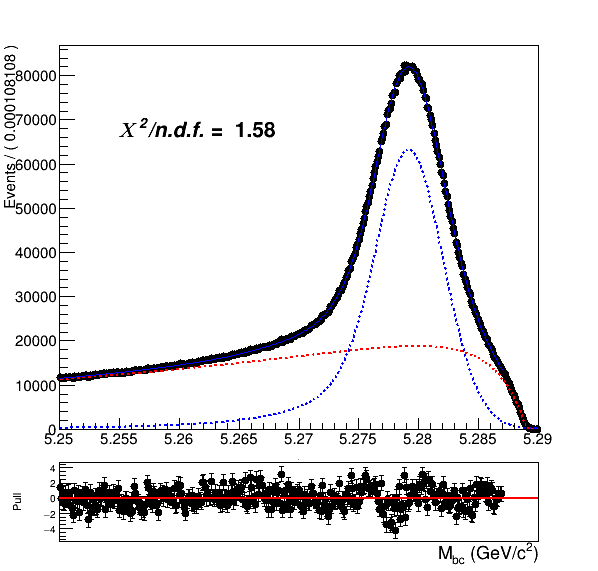
\includegraphics[width=0.40\textwidth]{06-Efficiencies/figs/stream5_chargedBtag_TotalSignal_addedGaussian_Normalisations.png}}
    \caption{Fitted distribution of tagged charged B mesons in the charged correlated
    decays sample.}
    \label{fig:stream5_chargedBtag_TotalSignal_addedGaussian_Normalisations}
    \end{figure}

 \subsection{Signalside-dependent FEI efficiency}

 The FEI tag-side efficiency for signal events is calculated upon 10 streams of on-resonance Monte Carlo streams of simulated data 
 in order to minimize statistical uncertainties.
 As an example \cref{fig:10streams_chargedBtag_corrLambdaC_TotalSignalBtag_fit} shows the fit performed on the tagged $B$ mesons having in the ROE a companion decaying $B^- \rightarrow \Lambda_c^+$ (charged correlated decays). 
 Dividing the yields obtained by the fit by the total number of $B^- \rightarrow \Lambda_c^+ events$ present in the 10 streams it is possible to determine the FEI tag-side efficiency for signal events.
 \begin{figure}[H]
    \centering
    {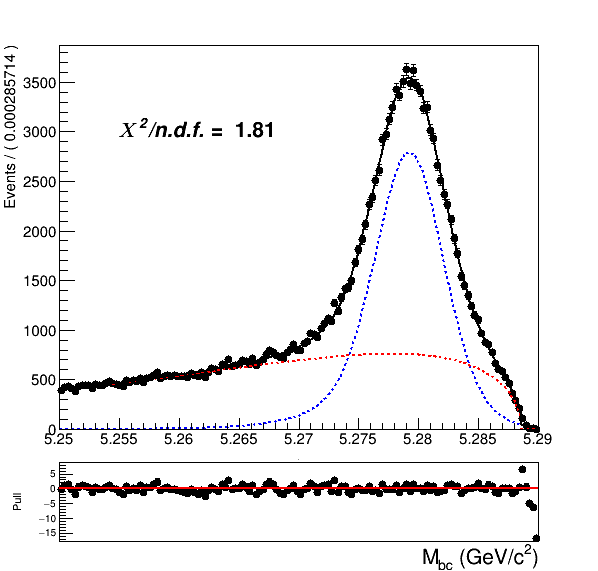
\includegraphics[width=0.40\textwidth]{06-Efficiencies/figs/10streams_chargedBtag_corrLambdaC_TotalSignalBtag_fit.png}}
    \caption{Fit of tagged $B$ mesons in the "signal events" sample}
    \label{fig:10streams_chargedBtag_corrLambdaC_TotalSignalBtag_fit}
    \end{figure}
\section{$\Lambda_c$ efficiency}
The efficiency of reconstructing the ${\Lambda_c}$ baryon after correctly tagging the charged $B$ meson, can be estimated from Monte Carlo simulated data.
All available 10 streams of on-resonance Monte Carlo streams of simulated data were used to minimize statistical uncertainties.
The efficiency is evaluated as follows from the fraction:  
\begin{equation}
    \frac{N_{recSig}(B_{tag}, \Lambda_c)}{N_{recSig}(B_{tag}^{sig})}
\end{equation}

\vspace{0.5cm}

\noindent where $N_{recSig}(B_{tag}, \Lambda_c))$ are the yields of reconstructed signal from a two dimensional fit of corresponding inclusive decay.
 and  $N_{recSig}(B_{tag}^{sig})$ are the yields of correctly reconstructed signal from the same fit of tagged $B$ mesons used to calculate the Signalside-dependent FEI efficiency. 

\subsection{$B^- \rightarrow \Lambda_c^+$ decays}
$\epsilon^+_{FEI,sig} = 0.636 \pm 0.003\%$ (calculated with 10 streams)\\
$\epsilon^+_{FEI} = 0.6379 \pm 0.0004\%$
$\frac{\epsilon^+_{FEI,sig}}{\epsilon^+_{FEI}}$ = 0.997 $\pm $ 0.005% 𝜖𝐹𝐸𝐼,𝑠𝑖𝑔= 0.636 ± 0.003% , 𝜖𝐹𝐸𝐼 = 0.638 ± 0.0004%

$\epsilon_{\Lambda_c}$ = 37.78 $\pm $ 0.45 $\%$ %correction factor: 0.969*0.853*0.983 = 0.813 ± 0.013

\subsection{$B^- \rightarrow \bar{\Lambda}_c^-$ decays}
$\epsilon^+_{FEI,sig} = 0.334 \pm 0.003\%$ (calculated with 10 streams)\\
$\epsilon^+_{FEI} = 0.3461 \pm 0.0002\%$
FEI calculation includes mixed events, $\epsilon_{\Lambda_c}$ is calculated without them
$\frac{\epsilon^+_{FEI,sig}}{\epsilon^+_{FEI}}$ = 0.965 $\pm $ 0.009% 𝜖𝐹𝐸𝐼,𝑠𝑖𝑔 = 0.334 ±0.003%  , 𝜖𝐹𝐸𝐼= 0.346 $\pm$ 0.0002%

$\epsilon_{\Lambda_c}$ = 42.39 $\pm $ 0.66 $\%$ %overall correction factor 0.794 ± 0.010


\subsection{$\bar{B^0} \rightarrow \Lambda_c^+$  decays}
$\epsilon^+_{FEI,sig} = 0.247 \pm 0.002\%$ (calculated with  10 streams unmixed)\\
$\epsilon^+_{FEI} = 0.236 \pm 0.0002\%$ (1 unmixed stream)

$\frac{\epsilon^+_{FEI,sig}}{\epsilon^+_{FEI}}$ = 1.056 $\pm$ 0.010% 𝜖𝐹𝐸𝐼=  0.234 ± 0.001% , 𝜖𝐹𝐸𝐼,𝑠𝑖𝑔= 0.247 ± 0.002%

$\epsilon_{\Lambda_c}$ = 39.59 $\pm $ 0.49 $\%$ %overall correction factor 0.794 $\pm$ 0.010
 (using unmixed events)

\subsection{$\bar{B^0} \rightarrow \Lambda_c^-$  decays}


$\frac{\epsilon^+_{FEI,sig}}{\epsilon^+_{FEI}}$ = 1.005 $\pm$ 0.014% 𝜖𝐹𝐸𝐼= 0.206 ± 0.001% , 𝜖𝐹𝐸𝐼,𝑠𝑖𝑔= 0.207 ± 0.003%

$\epsilon_{\Lambda_c}$ = 41.49  $\pm $ 1.13 $\%$ %overall correction factor 0.790 $\pm$ 0.011